\subsubsection{Controller PID}
\label{PID}

Per permettere al robot di seguire in maniera fluida il tracciato è stato implementato un controllo PID come illustrato in figura 4.

\begin{figure}[h!]
\centering
\begin{tikzpicture}[->, >=stealth', shorten >=0.1pt, auto, node distance=2cm, semithick,
								  hv path/.style={to path={-| (\tikztotarget)}},
								  tip/.style={->,shorten >=0.007pt}, 
								  vh path/.style={to path={|- (\tikztotarget)}}]

%====Definizione stile stati===============================================

	\tikzstyle{sommatore} = [circle, draw, text centered,  minimum width =0.02cm]
  	\tikzstyle{block}			=	[rectangle, draw, text centered, minimum height =1cm]
  	\tikzstyle{line} = [, draw]
%====Definizione stati e posizione==========================================
	\node[] 					(A) [label = set point]                   		{};
	\node[sommatore]  (B) [right of=A, node distance = 3cm, label = -240:$+$,label = -120:$-$]		{$\sum$};			
	\node[block]			(C) [right of=B, node distance = 3cm ]		{\textsc{pid}};
  	\node[sommatore] 	(D) [right of=C,node distance = 	3cm 	]		{} ;
  	\node[]         			(E) [right of=D,node distance = 	3cm, label = 90:uscita, label =- 90: velocita motori]  		{};
 	\node[]         			(F) [below of=B]  	{};
  	\node[]         			(G) [below of=D]  	{};
  	\node[block]         	(H) [below of=C]  	{\textsc{sensori di linea}}; 	
%====Definizione chain==================================================
    
       \path	 	(A) edge (B)
        			 	(B) edge node{errore}(C)
        				(C) edge (D);
        { [start chain]
        \chainin	(D) [join];
        { [start branch=minus]
        	\chainin (H) [join=by {vh path,tip}];
        	\chainin (B) [join=by {hv path,tip}];
        }
		\chainin(E) [join];				
    }				
\end{tikzpicture}
\caption{Schema a blocchi \textsc{PID}}
\end{figure}

\noindent Tale controllo agisce sulla velocità delle singole ruote apportando una correzione che dipende dall'errore e dai guadagni $K_p$, $K_d$, $K_i$ determinati sperimentalmente.
 L'attribuzione di un valore a questi parametri ha richiesto numerosi test, data la loro elevata influenza sull'andatura del robot. Poiché alcuni di essi risultano migliori per un determinato tracciato piuttosto che un altro si è cercato di trovare il compromesso che garantisse una maggiore flessibilità nell'affrontare differenti percorsi.
Tali guadagni permettono di calcolare la correzione da apportare ai motori mediante la seguente equazione \ref{eq}:
\begin{equation}
\label{eq}
PID_{value}=K_p\,e(t)+K_d\,\frac{de(t)}{dt}+K_i\int_0^te(\tau)d\tau
\end{equation}
Grazie a questo controllo il robot viene mantenuto allineato al percorso come si può graficamente apprezzare in un esempio di figura 5.

\begin{figure}[htb]
\centering
\label{PIDimage}
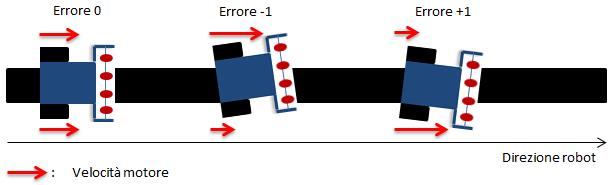
\includegraphics[width=0.65 \textwidth]{PID.jpg} 
\caption{Esempio correzione mediante \textsc{PID}}
\end{figure}

\subsubsection{Riconoscimento incroci e curve ad angolo retto}
Un incrocio viene individuato quando tutti i sensori rilevano la linea.
In tale condizione all'utente viene richiesto, mediante apposito comando, di scegliere la direzione da far intraprendere al robot. \\
Un problema particolare si è presentato nel riconoscimento delle curve ad angolo retto nelle quali, i sensori di linea, a causa della velocità del robot, uscivano brevemente dal tracciato perdendone la lettura.
Per garantire comunque una velocità sostenuta del robot è stato necessario dotare il sistema di una memoria che tenesse conto della direzione di uscita e ne garantisse il rientro dalla parte corretta. 
\subsection{Manual Control}
In tale modalità l'utente può controllare da remoto il robot tramite la connettività bluetooth.
Mediante l'utilizzo della tastiera del Pc è possibile guidare il robot nelle 4 direzioni principali agendo direttamente sui motori.
Il sistema garantisce continuamente un controllo attivo della presenza ostacoli ed in tale condizione ignora un comando errato dell'utente invertendo il moto ed evitando la collisione.
\subsubsection{Trasmissione comandi da remoto}
Per l'interfaccia con l'utente si è deciso di non utilizzare il serial monitor dell'ambiente Arduino ma di utilizzare il terminale Putty che permette un invio sequenziale dei comandi senza richiedere la pressione del tasto Enter. 